% =============================================================================
% FILE NAME : 00_introduction.tex
% DEPARTMENT: University of Tuebingen
% AUTOR     : Paul Palomero Bernardo & Konstantin Lübeck
% =============================================================================
% CONTENT   : Include for chapter "Introduction"
% =============================================================================
Beginnen sollte die Arbeit mit einer kurzen Einführung und Motivation in das Themengebiet. Aus der Motivation lassen sich ggf. bestehende Probleme ableiten bzw. Probleme aufzeigen, die man in dieser Arbeit lösen möchte. Danach erfolgt die Beschreibung der Aufgabenstellung.

Die Arbeit gliedert sich dazu wie folgt: Die Grundlagen von BlaBlaBla 
werden in Kapitel \ref{cha:fundamentals} erarbeitet. 

\section{Einige LaTeX-Hinweise}

Im folgenden wird das Einbinden einer Abbildung als `pdf-Datei' in ein
\LaTeX-Dokument gezeigt.

\begin{figure}[H]
	\centering
	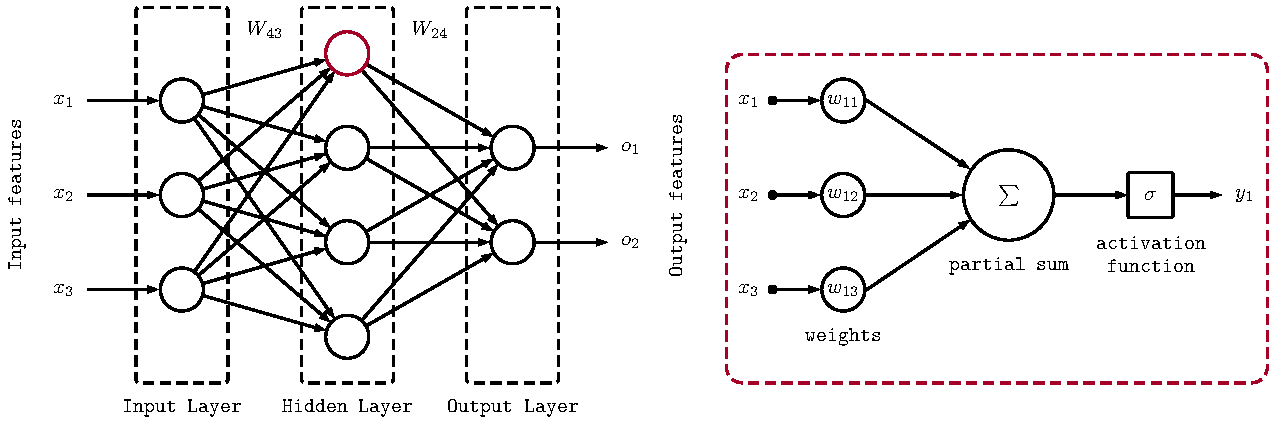
\includegraphics[width=\linewidth]{figures/example_fig.pdf}
	\caption[Schematic view of a simple MLP.]{Schematic view of a simple \gls{mlp}.}
  \label{fig:mlp}
\end{figure}

Abbildung \ref{fig:mlp} zeigt ...

Tabelle \ref{tab:tabelle_1}

\begin{table}[htb]
  \centering
  \begin{tabular}{p{2.7cm}lcr}
    \toprule
    \textbf{Spalte 1} 
    & \textbf{Spalte 2} 
    & \textbf{Spalte 3} 
    & \textbf{Spalte 4} \\
    \midrule
    xxx1111
    & xxxxxxx2222222
    & xxxxxx333333 
    & xxxxxxxxxx444444 \\

    yyy1111
    & yyyyyyy2222222
    & yyyyyy333333 
    & yyyyyyyyy444444 \\
    \addlinespace 

    zzz1111
    & zzzzzzz2222222
    & zzzzzz333333 
    & zzzzzzzzz444444 \\

    ...
    & ...
    & ...
    & ...\\
    ...
    & ...
    & ...
    & ...\\
    \bottomrule
  \end{tabular}
  \caption[Beispieltabelle mit langer Legende]{Beispieltabelle mit einer langen Legende, damit man sieht, dass in der Legende der Zeilenabstand verringert wurde. Außerdem soll auch der Font etwas kleiner gewählt werden. So sieht die ganze Umgebung kompakter aus.}
  \label{tab:tabelle_1}
\end{table}

Eine Aufzählung geht wie folgt:
\begin{itemize}
	\item ...
	\item ...
\end{itemize}
Eine nummerierte Aufzählung:
\begin{enumerate}
	\item ...
	\item ...
\end{enumerate}

Quellcodeauszug \ref{code:example}
\begin{lstlisting}[style=colorEX,language=PythonPlus,caption={Beispielcode},label={code:example}]
if __name__ == "__main__":
    print("Hello World!")
\end{lstlisting}


Betonungen sollen \emph{kursiv} gedruckt werden. 
\textbf{Fettdruck} ist auch möglich.

Zitieren einer Webseite \cite{webpage}.

SI Einheiten \SI{32}{\bit}, \SI{64}{\kilo\byte}, \SI{3.14}{\milli\watt}.


\section{Umfang der Arbeit}
,,Dies ist eine der meistgestellten Fragen. Natürlich verbirgt sich dahinter die Vermutung, die erzielbare Note sei – gutachterabhängig – mit der Seitenzahl korreliert (vgl. Abb.~\ref{fig:graph}). Nur
wie? Linear, normalverteilt, nach dem Gesetz vom abnehmenden Grenznutzen?
Tatsächlich kommt es auf die Qualität Ihrer Resultate an. Wenn Sie mit Ihrer Arbeit das Collatz-Problem, auch bekannt als Ulams Vermutung, widerlegen können, genügt eine Seite Inhalt mit dem Hinweis, die Zahl, welche die Vermutung widerlegt, befinde sich auf der beigefügten CD.

\begin{figure}[htb]
  \centering
  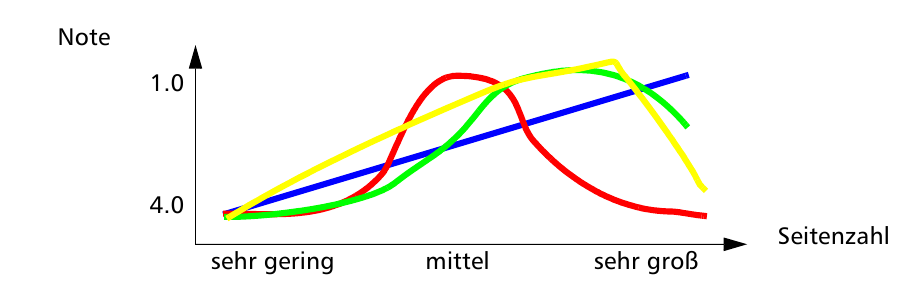
\includegraphics[width=0.9\textwidth]{figures/note_page.png}
  \caption[Verteilung: Seitenanzahl-Note]{Welcher Verteilung folgt die Note als Funktion der Seitenzahl?}
  \label{fig:graph}
\end{figure}

Für alle, die nicht so viel Glück haben, soll die folgende Tabelle \ref{tab:tabelle-2} auf Seite \pageref{tab:tabelle-2} als Richtschnur
dienen. Dabei wurden Anhänge, Inhalts- und Abbildungsverzeichnisse sowie Stichwortverzeichnisse (sofern überhaupt vorhanden, da nicht üblich) nicht gerechnet.Bedenken Sie, dass Ihr Gutachter das alles gründlich lesen soll, der Zweitgutachter es vielleicht
auszugsweise lesen muss. Formulieren Sie deshalb knapp und auf den Punkt, vermeiden Sie Wiederholungen („Wir kommen nochmal auf das schwierige Problem der Softwareauswahl aus
Kapitel zwei zu sprechen, wo wir feststellten, dass ...“).
Längliche Passagen, etwa Programmstücke, Teile der Dokumentation, sehr lange Zitate (etwa ein Beweis, ein Gerichtsurteil, ein Zeitschriftenartikel im Wortlaut), Messreihen usw.
verbannen Sie in den Anhang (mit der Gewissheit, dass das kaum jemand gründlich lesen wird).
Aber auch bei den Anhängen ist weniger oft mehr. Noch umfangreichere Teile lassen sich auf
eine CD brennen, die der Arbeit beigefügt wird; allerdings ist umstritten, ob ein Gutachter sich
diese anschauen muss.

\begin{table}[tb]
  \centering
  \begin{tabular}{cccc}
    \toprule
    \textbf{Art der Arbeit} & \textbf{Untergrenze} & \textbf{Obergrenze} & \textbf{Anmerkung} \\
		\midrule
    Bachelor & 35 & 65 & ideal $\leq$ 50 \\
    Master & 50 & 85 & ideal $\leq$ 70 \\
    \bottomrule
  \end{tabular}
  \caption{Empfehlung zur Seitenanzahl der Arbeit}
  \label{tab:tabelle-2}
\end{table}


Weil das Vorwort, der erste Abschnitt der Einleitung und die abschließende Zusammenfassung mit Ausblick immer gründlich gelesen werden, sollten Sie darauf besonderes Augenmerk
legen. In der Regel schreibt man die Einleitung und das Vorwort auch erst, wenn der restliche
Teil einschließlich Zusammenfassung (Fazit) steht, Spötter nennen das die Anpassung des
Anforderungsprofils an das tatsächlich erzielte Resultat.
Zuletzt ein Rat, wenn der Umfang der Arbeit erkennbar zu groß wird. So wie bei Seminarvorträgen Schnellersprechen das Problem eines zu umfangreichen Folienprogramms nicht
lösen kann, so wenig lässt sich mit typografischen Mitteln (kleinerem Font, engeren Zeilenabständen, breiteren Spalten) wesentlich Platz ohne Verlust an Lesbarkeit gewinnen. Sie kommen
nicht umhin, größere Teile der Arbeit zu streichen oder wesentlich zu straffen.
Dafür bieten sich oft die Kapitel an, in denen Sie den mühsamen Prozess der Lösungsfindung
einschließlich aller notwendigen Vorarbeiten und Diskussionen mit dem Anwender dokumentiert haben. Hinter solchen längeren Beschreibungen steckt der verständliche Wunsch, der Gutachter möge honorieren, dass Sie unglaublich mit dem Auftraggeber, der undurchsichtigen
Software, dem abstürzenden Computer u.a.m. kämpfen mussten und vieles zunächst nicht so
funktionierte, wie gedacht.
Leser sind aber wie Restaurantgäste, Gutachter ähneln Gourmetkritikern. Sie sind mitleidslos und schauen nur auf den Teller vor sich. Sie wollen nichts davon wissen, dass frische Seezunge heute enorm schwierig zu beschaffen war und der Jungkoch sich am Gratin die Finger
verbrannt hat. Halten Sie Ihre Schwierigkeiten in einem ehrlich geschriebenen 10-Zeilen-Abschnitt der Zusammenfassung fest, als Teil der Selbstreflektion, die immer zu einer
Abschlussarbeit gehört, und streichen Sie schweren Herzens Teile der Entwicklungssaga.''
